\documentclass[12pt]{article}

\usepackage{sbc-template}
\usepackage[utf8]{inputenc}
\usepackage[T1]{fontenc}
\usepackage[brazilian]{babel}
\usepackage{graphicx}
\usepackage{booktabs}
\usepackage{amsmath}
\usepackage{url}
\usepackage{microtype}
\usepackage{float}

\graphicspath{{figures/}}

\title{O Custo da Granularidade Semântica na Detecção de Resíduos:\
um Estudo Controlado com TACO e YOLO26n}

\author{Jean Carlos Rodrigues Sousa\inst{1}, Karielly de Carvalho\inst{1},
  Marcos A. G. B. Brito\inst{1}}
\address{Universidade Federal do Piauí (UFPI)\\
  Campus Senador Helvídio Nunes de Barros (CSHNB)\\
  Picos -- PI -- Brasil
  \email{\{jean.rodrigues, karielly.carvalho, marcos.brito\}@ufpi.edu.br}
}

\begin{document}
\raggedbottom

\maketitle

\begin{resumo}
A detecção de resíduos em cenas não controladas combina localização com uma decisão semântica cuja dificuldade depende da taxonomia. Este trabalho quantifica esse custo no TACO usando as mesmas imagens e caixas em três taxonomias: 60 classes detalhadas, seis grupos por material e uma classe para resíduo. Modelos YOLO26n foram treinados sob protocolo idêntico com três sementes e avaliados em teste fixo. O AP$_{50}$ médio foi $0{,}146\pm0{,}022$, $0{,}183\pm0{,}023$ e $0{,}567\pm0{,}002$ para Fine, Material e Binary. Entre modelos treinados separadamente, o bootstrap sustentou a melhora de Material em $F_1$, mas a diferença de AP permaneceu inconclusiva em duas sementes. Ao julgar as mesmas detecções Fine com rótulos mais amplos, o AP$_{50}$ passou de $0{,}103\pm0{,}007$ para $0{,}171\pm0{,}015$ no nível de material e $0{,}466\pm0{,}014$ sem distinção de classe; esses ganhos foram sustentados nas três sementes. No limiar de confiança 0,25, $56{,}95\pm1{,}38\%$ dos casamentos espaciais tinham classe Fine incorreta e $404{,}7\pm10{,}6$ dos 637 objetos foram omitidos. Classes raras obtiveram AP e revocação inferiores. Os resultados caracterizam a discriminação semântica sob cauda longa como um gargalo importante, coexistente com falhas espaciais; a taxonomia por material constitui um compromisso útil, embora sua superioridade em AP não seja estatisticamente definitiva.
\end{resumo}

\section{Introdução}

Detectar resíduos em ambientes externos é diferente de reconhecer itens em condições controladas: os objetos podem ser pequenos, deformáveis, transparentes, ocluídos ou visualmente confundidos com o fundo. O TACO (\textit{Trash Annotations in Context}) foi criado para representar esse cenário, reunindo fotografias de ambientes diversos e uma taxonomia hierárquica de resíduos \cite{proenca2020taco}. Entretanto, sua versão oficial contém apenas 1.500 imagens e 4.784 instâncias distribuídas em 60 categorias, combinação que impõe simultaneamente poucos dados e forte desbalanceamento.

Em detecção multiclasse, uma caixa espacialmente correta é considerada erro quando recebe a classe errada. Assim, o desempenho pode diminuir tanto por falhas de localização quanto pela exigência de distinguir categorias visualmente próximas e pouco representadas. A granularidade da taxonomia determina quanta informação semântica se exige do modelo, mas comparações entre estudos costumam misturar arquiteturas, partições e agrupamentos diferentes. Isso impede atribuir a variação de desempenho apenas aos rótulos.

Este trabalho investiga: \emph{como a granularidade das classes afeta a detecção de resíduos em um conjunto pequeno e de cauda longa, e quanto da perda decorre de localização versus discriminação semântica?} Para isolar essa variável, fixamos imagens, caixas, partição e protocolo de treino, alterando somente a taxonomia: Fine (60 classes oficiais), Material (seis macroclasses) e Binary (uma classe \textit{Litter}). Empregamos o YOLO26n, variante compacta da família YOLO26 \cite{jocher2026yolo26}, sem modificar sua arquitetura.

As contribuições são: (i) comparação controlada dos três níveis com três sementes; (ii) avaliação hierárquica das \emph{mesmas} predições Fine, remapeadas para material e para classe única; (iii) intervalos de confiança por bootstrap pareado por imagem, repetidos independentemente para cada semente; e (iv) análises multissemente de cauda longa e uma decomposição auditável dos erros. Todo número apresentado é produzido por scripts a partir das anotações, configurações, checkpoints ou predições salvas.

\section{Trabalhos Relacionados}

Proença e Simões \cite{proenca2020taco} introduziram o TACO com 60 categorias pertencentes a 28 supercategorias. Reconhecendo a ambiguidade visual e o desbalanceamento, os autores avaliaram Mask R-CNN em TACO-1, sem classes, e TACO-10, com nove supercategorias frequentes e uma classe residual. O agrupamento de rótulos no TACO, portanto, já foi explorado. O presente estudo distingue-se pela definição de três níveis ordenados, pela inclusão de um nível intermediário por material e pela reavaliação hierárquica das mesmas detecções para separar localização e semântica.

Córdova et al. \cite{cordova2022litter} compararam Faster R-CNN, Mask R-CNN, RetinaNet, EfficientDet e YOLOv5 em TACO e PlastOPol, relatando dificuldades com objetos pequenos e cenários naturais complexos. O estudo evidencia a relevância de detectores YOLO leves, mas os resultados não são diretamente comparáveis aos obtidos neste trabalho, pois diferem em taxonomia, partição, versão dos modelos e protocolo experimental. O objetivo da presente investigação não consiste em estabelecer o estado da arte, mas em mensurar uma variável experimental sob condições controladas.

YOLO surgiu como detector de estágio único orientado a inferência em tempo real \cite{redmon2016yolo}. O YOLO26 unifica modelos atuais da Ultralytics e oferece uma cabeça \textit{end-to-end} sem NMS, além de mecanismos de atribuição voltados a objetos pequenos \cite{jocher2026yolo26}. A variante nano foi selecionada por sua compatibilidade com uma GPU de 6~GB; não foi realizada comparação entre arquiteturas.

Em aprendizado visual, \emph{cauda longa} descreve a distribuição de frequência dos rótulos: poucas classes de ``cabeça'' concentram grande parte das amostras, enquanto muitas classes da ``cauda'' têm poucos exemplos \cite{cui2019classbalanced}. O termo se refere, portanto, ao desbalanceamento entre classes, não ao tamanho dos objetos nas imagens. Em detecção e segmentação de grande vocabulário, o LVIS demonstrou que essa escassez está associada a desempenho inferior nas categorias pouco representadas \cite{gupta2019lvis}. Perdas balanceadas por classe constituem uma estratégia de mitigação \cite{cui2019classbalanced}. No presente estudo, amostragem e função de perda foram mantidas inalteradas para evitar fatores experimentais adicionais; o desempenho foi mensurado nos estratos raro, médio e frequente.

Diagnósticos de detectores também requerem a separação entre classificação, localização, duplicatas, fundo e omissões. Essa motivação é formalizada pelo TIDE \cite{bolya2020tide}. A decomposição adotada utiliza categorias análogas, mas emprega um procedimento próprio de casamento guloso e deve ser interpretada como análise descritiva no limiar selecionado.

\section{Metodologia}

A Figura~\ref{fig:pipeline} sintetiza o desenho experimental. A partir de uma única versão auditada do TACO, mantemos a partição e as caixas constantes, derivamos três taxonomias, treinamos cada uma sob protocolo idêntico e aplicamos cinco análises complementares no mesmo conjunto de teste.

\begin{figure}[H]
  \centering
  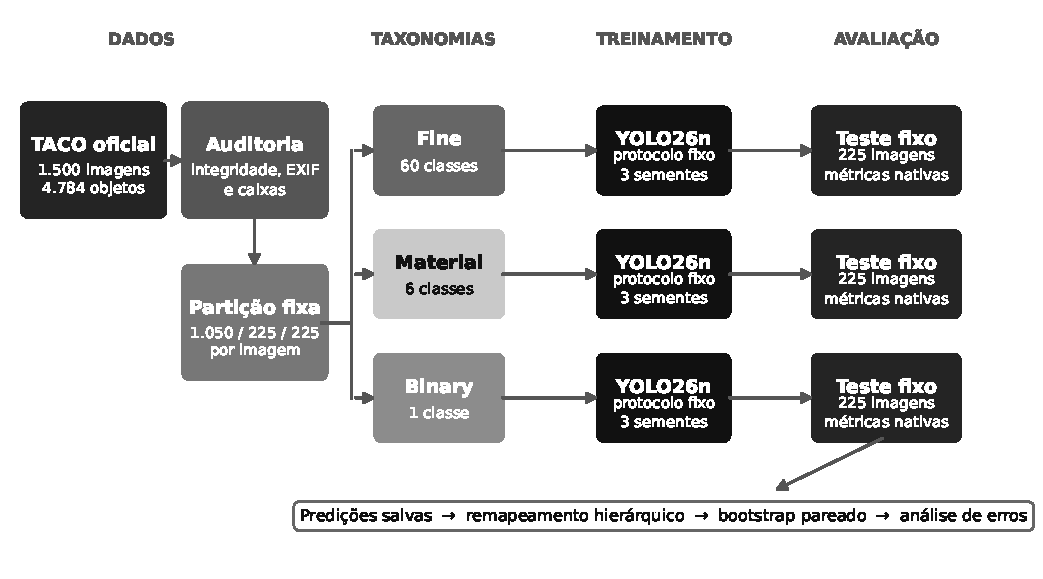
\includegraphics[width=.94\linewidth]{methodology_pipeline.pdf}
  \caption{Pipeline experimental. Somente a taxonomia varia entre os três ramos de treinamento; imagens, caixas, partição, arquitetura e hiperparâmetros permanecem fixos.}
  \label{fig:pipeline}
\end{figure}

\subsection{Dados, auditoria e partição}

Usamos exclusivamente \texttt{data/annotations.json} do repositório oficial TACO, em formato COCO \cite{lin2014coco}, e somente \textit{bounding boxes}. A auditoria programática confirmou 1.500 imagens, 4.784 objetos, 60 categorias, nenhuma imagem vazia e nenhum arquivo ausente. Sete caixas excediam a borda em no máximo 1,32 pixel; elas foram recortadas apenas na conversão, mantendo o JSON oficial intacto e registrando cada alteração.

A partição foi sorteada uma vez por imagem com semente 42: treino, validação e teste receberam, respectivamente, 1.050/225/225 imagens e 3.359/788/637 objetos. As três taxonomias reutilizam exatamente essa partição. As coordenadas COCO $(x,y,w,h)$ foram convertidas para centro, largura e altura normalizados do YOLO; scripts verificaram limites, dimensões positivas, IDs e igualdade das partições. Imagens com orientação EXIF foram transpostas fisicamente antes da conversão.

\begin{figure}[H]
  \centering
  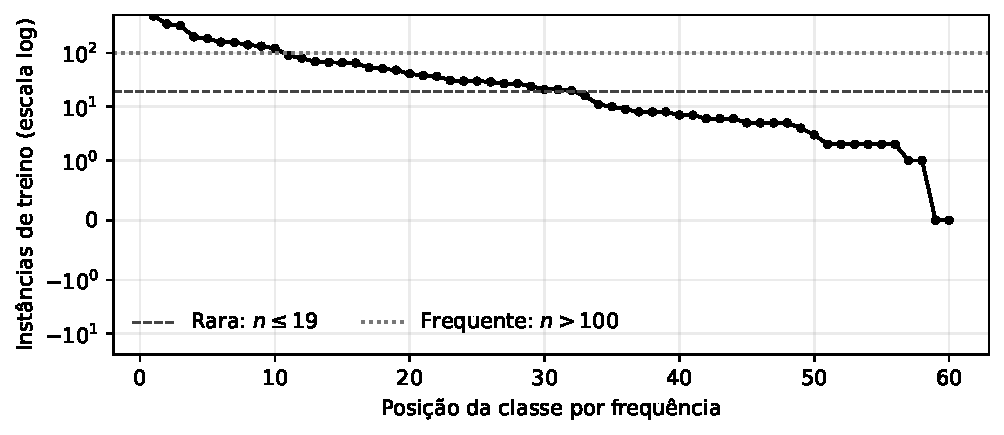
\includegraphics[width=.94\linewidth]{class_rank_distribution.pdf}
  \caption{Instâncias de treino das 60 classes Fine, ordenadas por frequência. As linhas marcam os limiares da análise de cauda longa.}
  \label{fig:distribution}
\end{figure}

\subsection{Taxonomias}

Fine preserva as 60 categorias oficiais. Material remapeia todas elas para Plastic (24 categorias de origem), Metal (9), Glass (4), Paper/Cardboard (13), Organic (1) e Other (9). Compostos ou itens sem associação natural, como bateria, sapato e embalagens multicamadas, foram enviados a Other; cada decisão e sua justificativa estão em \path{configs/material_mapping.json}. Binary atribui \textit{Litter} a todas as instâncias. As caixas não mudam entre versões. A Figura~\ref{fig:distribution} evidencia a cauda longa que motiva os agrupamentos.

\subsection{Modelo e protocolo experimental}

Treinamos YOLO26n inicializado com pesos COCO, entrada $640\times640$, lote 24, até 60 épocas, \textit{early stopping} com paciência 15, AdamW \cite{loshchilov2019adamw} e taxa inicial $10^{-3}$. Foram mantidas as transformações padrão da implementação Ultralytics, precisão mista e determinismo. Todos os experimentos usaram Python 3.12.10, PyTorch 2.8.0+cu128 e Ultralytics 8.4.157 em uma RTX 3060 Laptop de 6~GB. As sementes 42, 123 e 2026 foram aplicadas às três taxonomias; não houve ajuste específico por configuração.

\subsection{Avaliação e incerteza}

No teste fixo, reportamos precisão, revocação, $F_1$, AP$_{50}$ e AP$_{50:95}$ da implementação Ultralytics; esta última média usa IoU de 0,50 a 0,95 em passos de 0,05. A Tabela principal apresenta média e desvio-padrão entre sementes.

Para decompor o erro, um avaliador controlado faz casamento guloso um-para-um em ordem decrescente de confiança e AP interpolado em 101 pontos. Para cada modelo Fine, preservamos caixas e escores, mas remapeamos predição e verdade-terreno para Fine, Material ou Binary. Como essa implementação não é numericamente idêntica ao avaliador nativo, seus valores só são comparados entre si.

Aplicamos bootstrap percentil pareado \cite{efron1993bootstrap} para obter ICs de 95\%. Fizemos 2.000 reamostragens das 225 imagens de teste, com reposição e os mesmos índices nos dois lados. O bootstrap usa as predições da semente 42; as outras análises agregam três sementes. Para cauda longa, a frequência é calculada apenas no treino: rara ($n\leq19$), média ($20\leq n\leq100$) e frequente ($n>100$).

\section{Resultados}

\subsection{Efeito da taxonomia}

A Tabela~\ref{tab:main} resume os modelos treinados. Material elevou o AP$_{50}$ médio de 0,146 para 0,183 e o $F_1$ de 0,232 para 0,296 em relação a Fine. Binary alcançou 0,567 de AP$_{50}$ e apresentou a menor variação entre sementes ($\sigma=0{,}002$). Esse ganho não constitui uma comparação de capacidade semântica equivalente: Binary só precisa separar resíduo de fundo.

\begin{table}[H]
  \centering
  \caption{Teste por taxonomia: média $\pm$ desvio-padrão de três sementes.}
  \label{tab:main}
  \resizebox{\linewidth}{!}{\begin{tabular}{lrrrrr}
\toprule
Taxonomia & $P$ & $R$ & $F_1$ & AP$_{50}$ & AP$_{50:95}$ \\
\midrule
Fine & 0.360$\pm$0.063 & 0.173$\pm$0.010 & 0.232$\pm$0.005 & 0.146$\pm$0.022 & 0.118$\pm$0.022 \\
Material & 0.387$\pm$0.050 & 0.241$\pm$0.012 & 0.296$\pm$0.006 & 0.183$\pm$0.023 & 0.131$\pm$0.023 \\
Binary & 0.750$\pm$0.050 & 0.491$\pm$0.018 & 0.593$\pm$0.004 & 0.567$\pm$0.002 & 0.405$\pm$0.005 \\
\bottomrule
\end{tabular}
}
\end{table}

O bootstrap separa média superior de evidência repetível. Embora Material tenha superado Fine em média nas três métricas, seus ganhos de AP tiveram IC95\% acima de zero em apenas uma das três sementes. O ganho de $F_1$, por outro lado, foi sustentado nas três. Portanto, os modelos treinados separadamente permitem afirmar uma melhora consistente em $F_1$, mas não uma superioridade inequívoca de AP.

\subsection{Localização versus semântica}

A Tabela~\ref{tab:hierarchy} quantifica a variação observada quando as \emph{mesmas} caixas e confianças produzidas pelo modelo Fine são avaliadas com menor granularidade semântica. Ao aceitar a macroclasse de material, AP$_{50}$ passou de $0{,}103$ para $0{,}171$; sem distinção entre classes, alcançou $0{,}466$. Como esta análise não envolve novo treinamento, o ganho estima a parcela da penalização associada aos rótulos, embora a alteração da macro-média impeça sua interpretação como contagem pura de erros semânticos. A Tabela~\ref{tab:bootstrap} apresenta a repetibilidade desse efeito entre sementes.

\begin{table}[H]
  \centering
  \caption{Mesmas predições Fine avaliadas em três níveis pelo avaliador controlado (média $\pm$ desvio-padrão).}
  \label{tab:hierarchy}
  \begin{tabular}{lrrr}
\toprule
Nível de avaliação & $F_1$ & AP$_{50}$ & AP$_{50:95}$ \\
\midrule
Fine & 0.168$\pm$0.016 & 0.103$\pm$0.007 & 0.082$\pm$0.005 \\
Material & 0.264$\pm$0.021 & 0.171$\pm$0.015 & 0.122$\pm$0.010 \\
Binary & 0.506$\pm$0.011 & 0.466$\pm$0.014 & 0.322$\pm$0.011 \\
\bottomrule
\end{tabular}

\end{table}

\begin{table}[H]
  \centering
  \footnotesize
  \caption{Síntese do bootstrap pareado nas três sementes.}
  \label{tab:bootstrap}
  \begin{tabular}{llrr}
\toprule
Comparação ($A-B$) & Métrica & $\overline{\Delta}\pm\sigma$ & IC exclui 0 \\
\midrule
Fine$-$Material & AP$_{50}$ & $-0{,}051\pm0{,}022$ & 1/3 \\
Fine$-$Material & AP$_{50:95}$ & $-0{,}029\pm0{,}023$ & 1/3 \\
Fine$-$Material & $F_1$ & $-0{,}074\pm0{,}027$ & 3/3 \\
Fine$\rightarrow$Material$-$Fine & AP$_{50}$ & $+0{,}068\pm0{,}012$ & 3/3 \\
Fine$\rightarrow$Material$-$Fine & AP$_{50:95}$ & $+0{,}039\pm0{,}010$ & 2/3 \\
Fine$\rightarrow$Material$-$Fine & $F_1$ & $+0{,}101\pm0{,}008$ & 3/3 \\
Fine$\rightarrow$Binary$-$Fine & AP$_{50}$ & $+0{,}345\pm0{,}016$ & 3/3 \\
Fine$\rightarrow$Binary$-$Fine & AP$_{50:95}$ & $+0{,}226\pm0{,}012$ & 3/3 \\
Fine$\rightarrow$Binary$-$Fine & $F_1$ & $+0{,}318\pm0{,}011$ & 3/3 \\
\bottomrule
\end{tabular}

\end{table}

Cada célula da Tabela~\ref{tab:bootstrap} apresenta ganho médio $\pm$ desvio-padrão e, entre parênteses, quantos ICs de 95\% excluem zero. Valores positivos favorecem a alternativa mais simples; 3/3 indica evidência repetida nas três sementes, enquanto 1/3 recomenda cautela. ``Fine como'' denota remapeamento das mesmas predições, sem novo treinamento.

\begin{figure}[H]
  \centering
  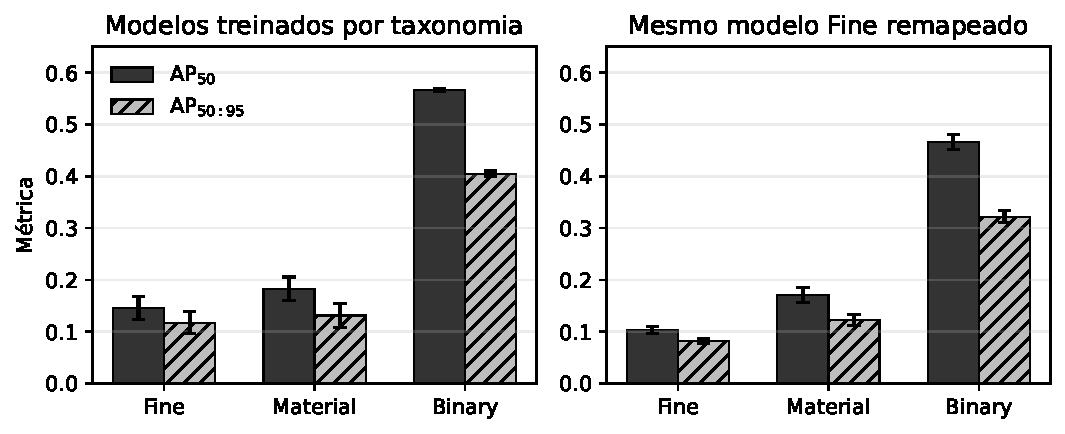
\includegraphics[width=\linewidth]{taxonomy_and_hierarchy.pdf}
  \caption{À esquerda, modelos treinados separadamente e avaliados pelo Ultralytics; à direita, mesmas predições Fine remapeadas e avaliadas pelo protocolo controlado. Barras de erro: um desvio-padrão entre sementes.}
  \label{fig:hierarchy}
\end{figure}

\subsection{Exemplos nos níveis Material e Binary}

A Figura~\ref{fig:model-level} amplia a análise visual para os demais modelos. Em (a), o modelo Material localiza e classifica corretamente um filme plástico. Os painéis (b) e (c) utilizam a mesma garrafa: o modelo Material preserva a localização, mas prediz Paper/Cardboard em vez de Plastic, enquanto o modelo Binary a identifica como \textit{Litter}. A comparação evidencia que a remoção da exigência de material pode converter uma confusão semântica em detecção correta. O painel (d) delimita esse efeito: apesar da ausência de distinção entre materiais, o modelo Binary omite um pneu de grandes dimensões no limiar de confiança 0,25. A redução da granularidade elimina determinados erros semânticos, mas não assegura cobertura espacial.

\begin{figure}[H]
  \centering
  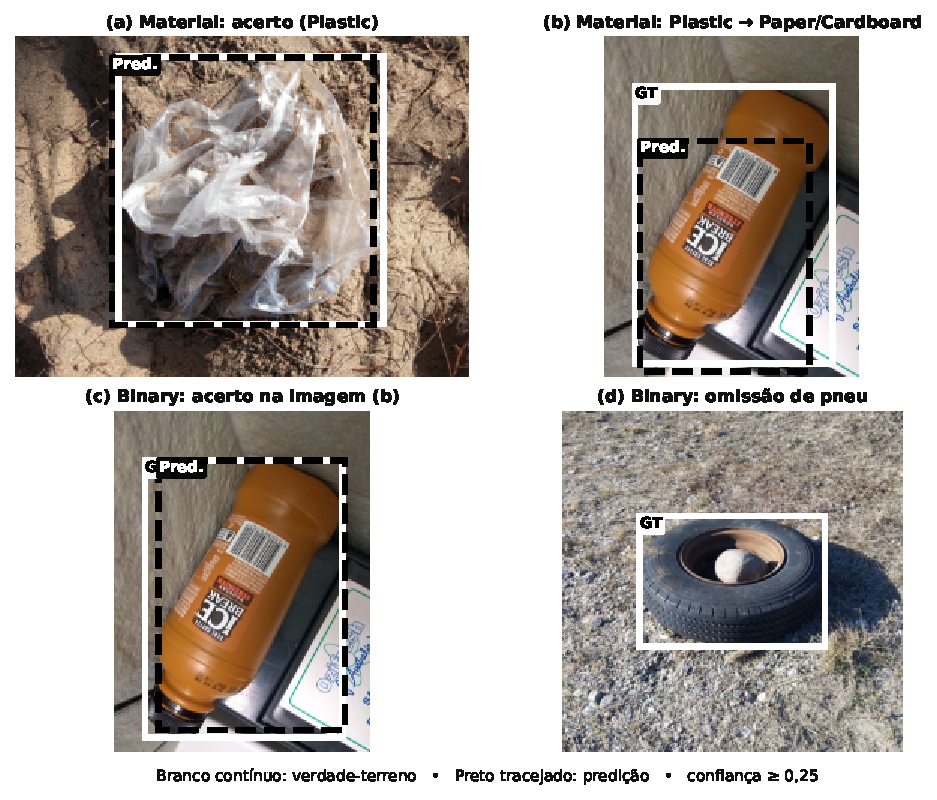
\includegraphics[width=.94\linewidth]{model_level_examples.pdf}
  \caption{Predições reais dos modelos Material e Binary, semente 42. Os painéis (b) e (c) mostram a mesma imagem sob duas taxonomias; (d) mostra uma omissão binária.}
  \label{fig:model-level}
\end{figure}

\subsection{Cauda longa e tipos de erro}

A Tabela~\ref{tab:tail} apresenta crescimento monotônico do desempenho com a frequência. Entre as classes presentes no teste, as raras obtiveram AP$_{50}=0{,}046$ e revocação $0{,}053$, enquanto as frequentes atingiram 0,207 e 0,282. Esse resultado indica que a dificuldade da taxonomia Fine não se distribui uniformemente entre os rótulos.

\begin{table}[H]
  \centering
  \caption{Desempenho Fine por frequência no treino, agregado em três sementes; somente classes com suporte no teste.}
  \label{tab:tail}
  \begin{tabular}{lrrrr}
\toprule
Grupo & \#classes & $n_{treino}$ & AP$_{50}$ & Recall \\
\midrule
Raras & 28 & 5.1 & 0.046$\pm$0.009 & 0.030$\pm$0.007 \\
Médias & 22 & 43.9 & 0.098$\pm$0.022 & 0.198$\pm$0.049 \\
Frequentes & 10 & 225.1 & 0.207$\pm$0.017 & 0.282$\pm$0.019 \\
\bottomrule
\end{tabular}

\end{table}

Como diagnóstico adicional, no limiar de confiança 0,25, as três sementes produziram $100{,}0\pm5{,}2$ acertos Fine e $132{,}3\pm7{,}2$ confusões semânticas entre $232{,}3\pm10{,}6$ casamentos espaciais. Portanto, $56{,}95\pm1{,}38\%$ dos casamentos em IoU$\geq0{,}5$ tinham classe Fine incorreta. Em média, houve ainda $16{,}3\pm5{,}5$ falhas de localização ($0{,}1\leq$IoU$<0{,}5$), $40{,}7\pm8{,}1$ duplicatas, $47{,}3\pm5{,}0$ falsos positivos de fundo (IoU$<0{,}1$) e $404{,}7\pm10{,}6$ objetos omitidos. Estes correspondem a $63{,}5\pm1{,}7\%$ dos 637 objetos de teste. Os totais dependem do limiar e servem para caracterização, não como substitutos das curvas de AP \cite{bolya2020tide}.

\begin{table}[H]
  \centering
  \small
  \caption{Decomposição dos erros Fine por semente no limiar de confiança 0,25. Categorias de predição e omissões são mutuamente exclusivas dentro de seus respectivos inventários.}
  \label{tab:errors}
  \begin{tabular}{lrrrr}
\toprule
Categoria & 42 & 123 & 2026 & Média $\pm$ DP \\
\midrule
Acerto Fine & 97 & 106 & 97 & $100{,}0\pm5{,}2$ \\
Confusão no material & 51 & 57 & 52 & $53{,}3\pm3{,}2$ \\
Confusão entre materiais & 73 & 79 & 85 & $79{,}0\pm6{,}0$ \\
Falha de localização & 11 & 16 & 22 & $16{,}3\pm5{,}5$ \\
Duplicata & 32 & 42 & 48 & $40{,}7\pm8{,}1$ \\
Falso positivo de fundo & 42 & 48 & 52 & $47{,}3\pm5{,}0$ \\
Objeto omitido & 416 & 395 & 403 & $404{,}7\pm10{,}6$ \\
\bottomrule
\end{tabular}

\end{table}

A Figura~\ref{fig:qualitative} liga essa decomposição às imagens de teste. A primeira linha apresenta o mesmo recorte sem anotações, com a verdade-terreno e com uma saída correta. Na segunda, uma lata é localizada corretamente, mas confundida com aerossol, preservando o material; uma embalagem metálica é confundida com papel/cartão; e uma tampa plástica anotada não recebe predição. Os exemplos tornam visíveis erros semânticos e espaciais de naturezas distintas.

\begin{figure}[!t]
  \centering
  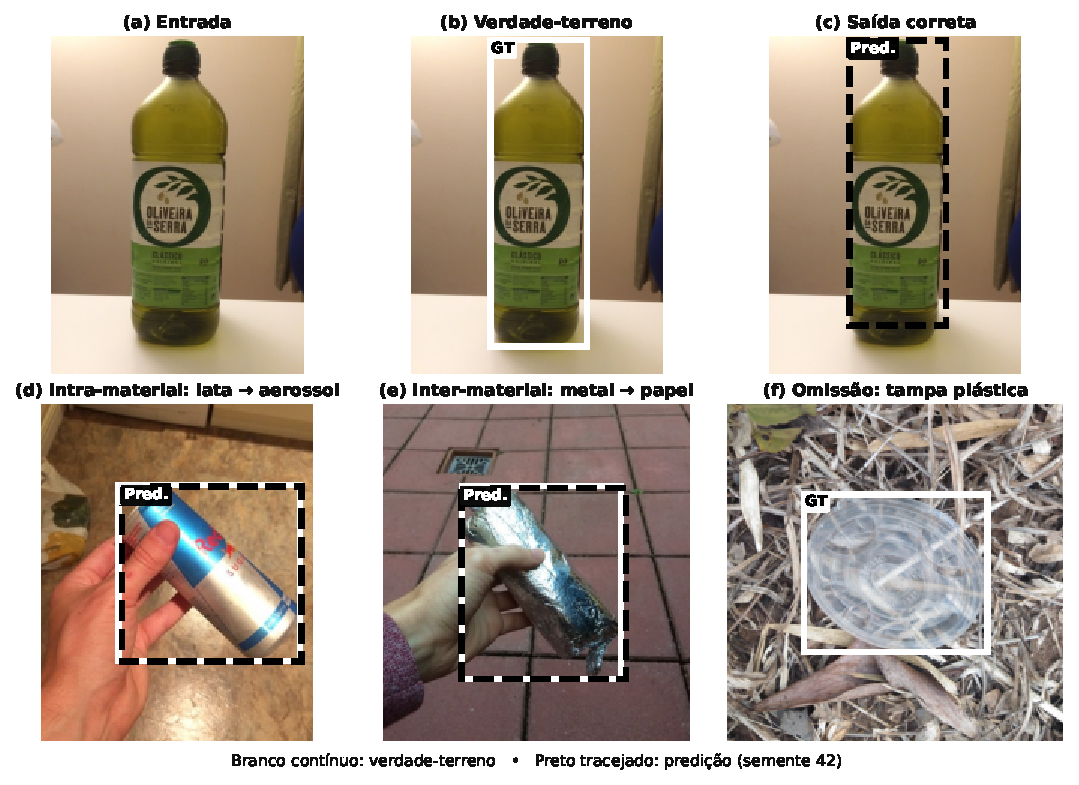
\includegraphics[width=.94\linewidth]{qualitative_analysis.pdf}
  \caption{Casos reais do teste Fine, semente 42. A primeira linha separa entrada, anotação e saída correta; a segunda exemplifica confusão intra-material, confusão inter-material e omissão. As imagens foram recortadas apenas para legibilidade; a prevalência de cada erro é quantificada nas três sementes na Tabela~\ref{tab:errors}.}
  \label{fig:qualitative}
\end{figure}

\section{Discussão}

Os resultados apoiam parcialmente a hipótese de que reduzir granularidade melhora a detecção. Material apresentou médias superiores a Fine, sobretudo em $F_1$, mas o IC pareado de AP inclui zero. Portanto, ``menos classes é melhor'' seria uma conclusão excessiva. Binary é claramente mais fácil, porém responde a outra pergunta operacional e perde toda informação sobre composição do resíduo.

A evidência mais forte vem da avaliação hierárquica. Quando uma caixa Fine recebe crédito após remapeamento, nenhuma propriedade geométrica ou confiança muda. O salto significativo nos dois níveis indica que muitas detecções contêm informação espacial útil, mas falham sob rótulos detalhados. Ainda assim, o AP binário controlado permanece abaixo de 0,5, e a decomposição registra muitas omissões; localização também está longe de resolvida.

A cauda longa oferece uma explicação complementar. As 28 classes raras têm, em média, somente 5,1 instâncias de treino e desempenho muito inferior às dez frequentes. Isso é consistente com a literatura de detecção de grande vocabulário \cite{gupta2019lvis}, mas aqui não demonstra causalidade isolada: tamanho, oclusão, contexto e semelhança visual também variam entre classes. A macroclasse Material compartilha dados entre rótulos relacionados e preserva uma informação potencialmente útil à triagem, constituindo compromisso plausível entre especificidade e robustez.

Há quatro ameaças principais à validade. Primeiro, uma única partição fixa não mede variação de amostragem; as três sementes medem somente a instabilidade de otimização. Segundo, o bootstrap cobre a semente 42 e condiciona-se ao teste observado. Terceiro, o mapeamento por material é uma decisão de projeto: compostos foram enviados a Other, e Organic contém apenas \textit{Food waste}. Quarto, não comparamos diretamente nossos números aos de trabalhos anteriores devido a diferenças de tarefa e protocolo. Estudos futuros devem repetir partições, avaliar agrupamentos alternativos e testar técnicas de balanceamento sem alterar simultaneamente outros componentes.

\section{Conclusão}

Os resultados indicam que a granularidade semântica impõe custo mensurável à detecção no TACO, embora não constitua seu único fator limitante. A taxonomia Material representa um compromisso defensável: preserva informação sobre composição e melhora o ponto operacional em relação a Fine, ainda que sua superioridade em AP não seja uniforme. Binary maximiza a detectabilidade ao custo da eliminação dessa informação. A avaliação das mesmas caixas, a decomposição de erros e a análise de cauda longa indicam, em conjunto, a coexistência de confusão semântica, escassez de exemplos e omissões espaciais. Portanto, a taxonomia deve ser selecionada segundo a informação requerida pela aplicação, e não apenas pela maior métrica. O fluxo experimental disponibiliza configurações, mapeamento integral, partição, predições, scripts e artefatos derivados para reprodução e extensão do estudo.


\bibliographystyle{sbc}
\bibliography{references}

\end{document}
